\documentclass[aps,pra,twocolumn,superscriptaddress,nofootinbib,10pt]{revtex4-2}

\usepackage{amsmath}
\usepackage{amssymb}
\usepackage{graphicx}
\usepackage{booktabs}
\usepackage{xcolor}
\definecolor{linkink}{rgb}{0.35,0.10,0.10}
\usepackage[colorlinks=true,allcolors=linkink]{hyperref}
\usepackage{microtype}

\begin{document}

\title{Patch or Reinterpret?\\
A Prize Corpus and a Measurable Test for the Move Models Do Not Make}

\author{Tianyu Wu}
\affiliation{Center for Biophysics and Quantitative Biology,
University of Illinois Urbana-Champaign, Urbana, Illinois 61801, USA}
\email{tianyu16@illinois.edu}

\date{\today}

\begin{abstract}
A breakthrough is rarely a better fit to the data nowadays. More often it is a decision that the data was
about something else. Lorentz and Einstein predicted the same numbers, and Einstein's theory
dropped an aether velocity no measurement could reach. Prusiner did not find the missing virus
behind scrapie---he proposed that the infectious agent had no genome. Cook and Karp did not find
faster algorithms for scheduling, colouring and satisfiability---they showed the problems were
one problem in disguise. Each time a repair was available that left the old description standing, and the move that won
discarded part of that description instead. Machine learning has no operation for that move, and
a language model retells these episodes fluently but, we find, cannot make the same call on a
case it does not recognise. We contribute three things. A \emph{framework}: what a discovering
system must be able to do, from fitting parameters up to introducing a kind of object its
language lacked. A \emph{corpus}: 2{,}327 prize records (1731--2026), 1{,}547 annotated by what
the contribution did---and the one move machine learning knows how to make appears in 131 of
them, while more than half the corpus does not change a description at all. And a \emph{test}: a theory's cost splits into structure it uses and structure no
measurement can see, both measured rather than declared, separating Einstein from Lorentz at
identical coverage and identical explanatory work. The annotations come from a language model
under human direction, not from domain experts; independent re-annotation is the most useful
thing a collaborator could contribute. Data, code and negative results are released together.
\end{abstract}

\maketitle

\section{Reinterpretation is the move that matters}

From the outside, science advances by measuring better and fitting better. From the inside, the
decisive step is usually something else: someone changes what the measurements are taken to be
about, and the old description loses a part it never needed.

In 1905 two theories fitted every optical and electrodynamic measurement equally well. Lorentz
kept absolute space and added a contraction hypothesis and a local-time auxiliary, so that the
aether became exactly undetectable~\cite{lorentz1904electromagnetic}. Einstein removed the
aether~\cite{einstein1905electrodynamics}. Nothing in the data chose between them: the choice was about which theory carried structure nothing could ever observe.

The shape is not peculiar to physics, and not confined to a century ago. Cook and Karp did not
find faster algorithms for scheduling, colouring and
satisfiability---they showed that these were one problem
wearing different clothes~\cite{cook1971complexity,karp1972reducibility}. Prusiner did not find
the slow virus behind scrapie---he proposed that the infectious agent carried no genome at all,
which meant admitting a kind of object biology's vocabulary did not
contain~\cite{prusiner1982prions}. Thouless and colleagues accounted for the quantum Hall
plateaus not with a better model of disorder but by recognising the conductance as a topological
invariant~\cite{thouless1982quantized}. Brangwynne and Hyman did not find the missing membrane around the
cell's P granules---they showed the granules were liquid drops, which meant accepting an
organelle that no membrane bounds~\cite{brangwynne2009granules}.

In every one of these a repair was available that would have left the existing description
standing---a hidden virus, a subtler disorder model, a membrane too faint to see---and in every one the
question was settled the other way. This is what we mean by reinterpretation, and it is what the
rest of the paper tries to make measurable.

The distinction itself is old: Kuhn separated normal science from
revolution~\cite{kuhn1962structure}, and Lakatos called an auxiliary that rescues a theory
without predicting anything new \emph{ad hoc}~\cite{lakatos1970falsification}. Both verdicts are
delivered in retrospect and in prose. What is missing is one that can be computed while the
outcome is still open.

Machine learning has no operation for this move either. Gradient descent searches within a fixed
description. A language model can recount the Lorentz--Einstein
episode in detail, but recounting is recall, and the open question is whether it can make the
call on a case it does not recognise. Section~\ref{sec:llm} reports that it largely cannot.

Progress needs two things that do not exist: real instances, and a test runnable without knowing
the answer. We offer both, plus a framework saying where they sit.

\begin{figure*}[t]
\centering
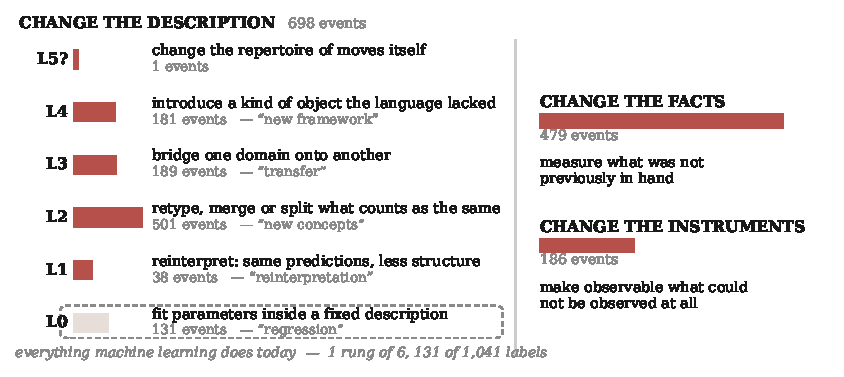
\includegraphics[width=\textwidth]{fig_framework.pdf}
\caption{What a discovering system has to be able to do. A move changes the facts you hold, the
instruments you have, or the description you use; a change to the description has a depth.
Counts are annotated prize events. Ordinary machine learning implements the bottom rung.}
\label{fig:framework}
\end{figure*}

\section{What awarded work actually did}
\label{sec:corpus}

The corpus does not count prizes; it labels each event by \emph{what the contribution did}. The
resulting distribution is this paper's main empirical finding, and it is what Table~\ref{tab:tax}
reports.

There are two axes. The first asks what changed. A contribution can put facts in your hands that
nobody had, extend what can be reached at all, build a thing that works, make something
computable, or change the description used to write the phenomenon down. Every event gets exactly
one of these, recording its primary move. The second axis is ordinal rather than nominal, and it
is defined only where a description changed, because only a description has a depth: a change can stay inside the language you already have, keep every prediction while
shedding structure, retype what counts as the same thing, bridge one domain onto another,
introduce a kind of object the language lacked, or alter the repertoire of moves itself.
Figure~\ref{fig:framework} draws both axes; Table~\ref{tab:tax} gives the counts and one real
award for each category. The two axes stay separate because they are different kinds of
measurement: no ordering holds between measuring something new and retyping what counts as the
same, whereas the rungs are ranked, and it is the ranking that carries the argument about machine
learning. The scheme is not symmetric about this---the facts column draws its own coarse
distinction, between facts newly in hand and reach newly extended, but encodes it as two modes
instead of a ladder. A scheme that graded every column would be cleaner, and we did not build
one.

\begin{table*}[t]
\caption{What 1{,}547 awarded contributions did, with one real award per category. Every event
receives exactly one mode, recording its primary move; a depth grade is added wherever a
description changed, which is why 820 events carry none. Depth is multi-label, so its 1{,}041
labels fall on 727 events---the 698 \textsc{represent} events plus 29 whose citation rewards a
second, description-changing move as well.}
\label{tab:tax}
\begin{ruledtabular}
\footnotesize
\begin{tabular}{lrl}
\textbf{Mode} --- what the contribution changed & $n$ & example \\
\colrule
\textsc{represent} \ the description used & 698 & Prusiner 1997---prions, ``a new principle of infection''~\cite{prusiner1982prions} \\
\textsc{record} \ facts nobody had & 479 & P\"a\"abo 2022---genomes of extinct hominins \\
\textsc{reach} \ what can be observed at all & 186 & Karik\'o and Weissman 2023---mRNA as a platform~\cite{kariko2005suppression} \\
\textsc{artifact} \ a thing that works & 102 & Goodenough \emph{et al.} 2019---the lithium-ion battery \\
\textsc{tractable} \ what can be computed & 32 & Hassabis and Jumper 2024---protein structure \\
\textsc{organize} \ a field's standing or reach & 11 & a field founded, legitimated or carried outward \\
\textsc{out-of-scope} \ not a scientific contribution & 31 & chiefly Templeton awards to religious figures \\
\textsc{unresolved} \ citation too thin to place & 8 & early Copley Medals, 1803--1824 \\
\colrule
\textbf{Depth} --- how far the description moved & $n$ & example \\
\colrule
\textbf{L0} \ inside the existing description & 131 & Duminil-Copin 2022---3D and 4D phase transitions \\
\textbf{L1} \ same predictions, less structure & 38 & Nambu 2008---symmetry breaking into particle physics \\
\textbf{L2} \ retype, merge or split & 501 & Cook 1982---NP-completeness~\cite{cook1971complexity} \\
\textbf{L3} \ bridge one domain onto another & 189 & Bennett and Brassard 2025---quantum communication \\
\textbf{L4} \ a kind of object the language lacked & 181 & Scholze 2018---perfectoid spaces \\
\textbf{L5} \ the repertoire of moves itself & 1 & Cohen 1966---forcing \\
\end{tabular}
\end{ruledtabular}
\end{table*}

Three results follow, and together they set the shape of the rest of the paper.

\paragraph{Most awarded work does not change a description at all.} Of the 1{,}547 events, 820
carry no depth grade, because the contribution delivered facts or reach instead. A split between
fitting and reinterpreting---the two moves this paper is about---would therefore miss more than
half of what gets awarded. This is why the framework has three columns rather than one axis, and
it is the main reason we do not treat reinterpretation as the whole of discovery.

\paragraph{Machine learning occupies one rung of six.} Work inside a fixed description, L0,
carries 131 of the 1{,}041 depth labels. That rung is not the shallow end---Duminil-Copin's
Fields Medal sits on it---but it is the only one for which machine learning has an operation, and
the five above it are populated by real awarded work rather than by speculation about what a
discovering system might one day do.

\paragraph{Strict reinterpretation is the rarest move in the corpus.} L1---same predictions,
less structure, Einstein against Lorentz---is 38 events, under 3\%. Most description-changing
work is L2, retyping what counts as the same thing, at 501 labels. The move this paper is named
after is not the common case but the extreme one, which is part of why a test for it is hard to
build and easy to fool.

\paragraph{What the corpus holds.} The release covers \textbf{2{,}327 award records} across
\textbf{23 prizes}, 1731--2026---the three science Nobels, the Copley Medal, Turing, Fields,
Abel, Wolf, Crafoord, Kavli, Shaw, Breakthrough and thirteen others---of which \textbf{2{,}221}
carry the awarding body's own citation. It also indexes 4{,}044 official documents and 15{,}693
laureate-to-paper links across 1{,}969 laureates. Sources are the Nobel Prize API, awarding-body
pages, Wikipedia and the Internet Archive, and every row records which one it came from. Of the
2{,}327 awards, 106 have no citation---never published rather than missed by us. Events also
carry labels from 39 operators: \textsc{add/remove latent object} (139), \textsc{map/transfer}
(135), \textsc{find invariant/symmetry} (110), and others. Existing prize datasets are
bibliometric---who won, what they published, how it was cited~\cite{li2019nobel}---which supports
questions about productivity but cannot say whether an advance reframed something or measured
something new. That distinction is what this corpus adds.

\paragraph{The annotations, and their central limitation.} They were produced by a large language
model (Claude, Anthropic) reading each official citation under human direction, in 13 batch files
shipped with the release. They are \emph{not} the judgements of human domain experts. There is
exactly one annotator, so no inter-annotator agreement statistic exists and we do not report a
proxy for one. Evidence grades---A (1{,}442), B (77), C (28)---are a confidence signal, not a
validation. The boundary that matters most is the one between \textsc{record} and
\textsc{represent}: a paper that reports a measurement often reframes something too, and which
half the citation rewards is a judgement call. Read the 820 as a lower bound on how badly a
two-way split fails, not as a constant.

\section{Telling a reinterpretation from a patch}

A patch and a reinterpretation both end up covering the anomaly, so what separates them is what
they cost---and a usable test needs a cost that whoever writes the theory down cannot
manipulate. We split the cost in two and measure both.
\textbf{Structure used} is the effective degrees of freedom, estimated by perturbing the data and
seeing how far the fit follows~\cite{ye1998gdf}; unlike a parameter count, this sees flexibility
hidden inside code. \textbf{Structure carried but unobservable} is the null space of the
prediction Jacobian---directions you could change without altering any prediction. That is
structural non-identifiability~\cite{raue2009identifiability}, read as a property of a theory
rather than a nuisance in a fit.

A patch adds structure; a reinterpretation removes it. Neither term is declared, so the encoding
does not control the verdict---a property we reached only after a description-length
score~\cite{rissanen1978mdl} gave the wrong answer on a case whose historical outcome is not in
doubt.

\begin{figure}[t]
\centering
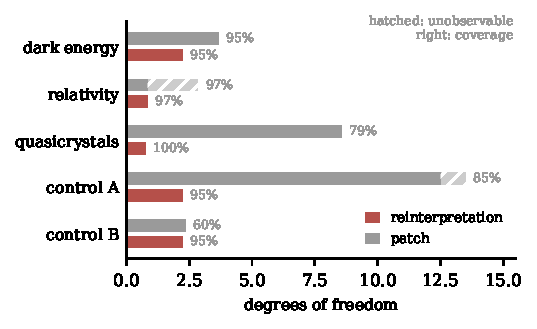
\includegraphics[width=\columnwidth]{fig_decomp.pdf}
\caption{Three historical episodes---each with the patch proposed at the time and the
reinterpretation that displaced it---plus two constructed controls. In the relativity row both
candidates fit 97\% of observations with identical effective work; the whole difference is two
directions nothing can measure.}
\label{fig:decomp}
\end{figure}

Figure~\ref{fig:decomp} applies this to three historical episodes, each encoded as competing
programs over real or reconstructed data: supernova distance moduli~\cite{scolnic2018pantheon}
for the acceleration reported in 1998--99~\cite{riess1998acceleration,perlmutter1999measurements}
against the grey-dust patch offered for the same dimming~\cite{aguirre1999dust}; relativistic
mass~\cite{einstein1905electrodynamics} against Lorentz's aether
theory~\cite{lorentz1904electromagnetic}; and quasicrystal
diffraction~\cite{shechtman1984quasicrystal} against Pauling's multiple
twinning~\cite{pauling1985twinning}. Table~\ref{tab:tax} places two of these prizes under
\textsc{record}, because the awards went to the observations rather than to the reframings that
followed; the corpus labels what a prize rewarded, while Fig.~\ref{fig:decomp} asks which of two
theories offered for one anomaly is the reinterpretation. Two controls check the test from the other side---a
degree-14 polynomial that fits by flexibility alone, and a theory tuned to the anomaly that
breaks what the old one had right.

The relativity row is the one to look at. Both theories cover 97\% of observations and both use
0.9 effective degrees of freedom---identical explanatory work. Lorentz's carries two directions
that change no prediction; Einstein's carries none. Nothing in the data distinguishes them; the
decomposition does.

\section{Can a language model make the call?}
\label{sec:llm}

We put the same five episodes to a 20B-parameter open-weight model~\cite{openai2025gptoss} in
three conditions: \textbf{named}, with
real theories and domain words; \textbf{blind}, every identifier alpha-renamed but fit statistics
retained; and \textbf{bare}, renamed with statistics withheld. In \emph{bare}, only the formulas
and their coverage remain.

\begin{table}[b]
\centering
\caption{Accuracy at identifying which of two candidates is the reinterpretation. Twelve repeats
per cell, presentation order randomised; the two controls are averaged. Chance is 50\%.}
\label{tab:llm}
\begin{ruledtabular}
\begin{tabular}{lccc}
episode & named & blind & bare \\
\colrule
dark energy & 67\% & 42\% & 50\% \\
relativity & 100\% & 100\% & 100\% \\
quasicrystals & 100\% & 50\% & 42\% \\
two controls & 84\% & 25\% & 38\% \\
\colrule
pooled, 60 trials & \textbf{87\%} & 48\% & 53\% \\
\end{tabular}
\end{ruledtabular}
\end{table}

Separating \emph{blind} from \emph{bare} matters: with statistics in view a model can score well
by reading off ``0 directions that change no prediction'', which is the test's answer rather than
the model's judgement. Accuracy is far above chance when the model can recognise the episode
($p=5{\times}10^{-9}$) and \emph{indistinguishable from chance} when it cannot ($p=0.9$ blind,
$0.7$ bare; named against blind, paired $p=0.03$). The model is recalling these episodes, not judging them---renaming alone is already known to
move accuracy on grade-school arithmetic~\cite{mirzadeh2025gsmsymbolic}, and the blind condition
is that probe applied to discovery. One case survives
anonymisation: relativity stays at 100\% because $(1-v^{2})^{-1/2}$ is recognisable from its
algebra whatever the identifiers are called. Handing over the statistics does not rescue the
others, so the failure is not a missing-information problem.

\section{What else we built, and what failed}

Two further components sit in the \emph{facts} column of Fig.~\ref{fig:framework}, and one of
them works. Nothing we built touches the \emph{instruments} column at all.

\paragraph{Changing the facts.} \textsc{Record} and \textsc{Reach} are 43\% of annotated events,
and the machine-learning form of the question is concrete: when error stops falling, is the
network too small or are the inputs insufficient? With outcomes measured $n$ times at one input,
$\mathbb{E}\lVert f(x)-y\rVert^{2}=\lVert f(x)-\mathbb{E}[y|x]\rVert^{2}+\mathrm{Var}(y|x)$, and
the second term is measured, so the model's own miscalibration cannot enter it. We built two worlds that give a small
network the same test error but differ in which limit binds. The measured floor recovers the true
irreducible share in both (1\% and 97\%). A Gaussian-likelihood variance
head~\cite{kendall2017uncertainties} and a deep ensemble~\cite{lakshminarayanan2017ensembles}
report 98\% in both---including the world where 99\% of the error is removable by a larger
network.

On CIFAR-10H, which supplies about 51 human labels per image~\cite{peterson2019cifar10h}, the
measured floor is 0.0765 and nine networks from 2.5\,K to 8.9\,M parameters all stay above it.
They also plateau at 0.194, well short of it, so the experiment shows the floor is never crossed
and not that capacity closes the gap to it.

\paragraph{Choosing what to measure next.} Ranking which unmeasured channel to acquire lost to
greedy forward selection. Automating the choice of \emph{which variable to measure} has been open
since the first robot scientists~\cite{king2004robot}, and we did not move it.

Each has an ancestor---Cascade-Correlation~\cite{fahlman1990cascor},
DreamCoder~\cite{ellis2021dreamcoder}, LaSR~\cite{grayeli2024lasr} on the Feynman
benchmark~\cite{udrescu2020feynman}---and we claim novelty for none, only reporting which
survived our own tests.

\section{Limitations, and what would help}

\paragraph{One annotator, and it is a model.} Every count in Fig.~\ref{fig:framework} is one
annotator's judgement, and that annotator is a language model under human direction. Independent
re-annotation of even a few hundred events would establish whether the scheme is reproducible or
whether we are reporting one system's habits.

\paragraph{The test was revised against known answers.} The criterion behind
Fig.~\ref{fig:decomp} was modified eight times, each after seeing a verdict we knew to be wrong,
each with a principled justification---which is what hindsight looks like from the inside. A
third clause meant to catch relabelling never changed a verdict across ten judgements. Five
episodes whose outcomes we knew establish internal consistency, not predictive power.

\paragraph{Hindsight and selection.} Prizes are awarded with decades of hindsight, so the corpus
samples work that turned out to matter, and citations justify a decision already taken. Physics
and mathematics are better represented than biology or the earth sciences.

\paragraph{What would help most.} Re-annotation by people who disagree with us. A case whose
answer nobody knows---a live controversy, or a synthetic episode with ground truth withheld,
since neither can be run by us alone without leaking what we know. And an attack on the untouched
rungs: L3 and L4 are 370 labels between them, and no system we know of has an operation for either. Predicate invention, the closest
existing target, is still open after three decades of inductive logic
programming~\cite{cropper2022ilp}.

\paragraph{Availability.} Data, annotations and code are released together under CC~BY~4.0 for
our annotations; the citation text remains the awarding bodies'.

\bibliographystyle{apsrev4-2}
\bibliography{refs}

\end{document}
